\documentclass{ctexart}

\usepackage{amsmath}

\usepackage{amsthm}

\usepackage{amssymb}

\usepackage{bm}

\usepackage{graphicx}

\usepackage{listings}
\lstset{
basicstyle=\scriptsize
}

\usepackage{caption}

\begin{titlepage}

\title{微分方程数值解 \\ 第三周作业}

\author{于慧倩 \\ 14300180118}

\date{2017年3月}

\end{titlepage}

\begin{document}

\maketitle

\newpage

\begin{enumerate}
%第一题

\item 演示Runge现象,并说明等距节点插值与Chebyshev多项式插值逼近的差异。


对函数\(f(x)= \displaystyle \frac{1}{1+25x^2}\)编写n次等距插值与Chebyshev插值程序,得到从n=3到n=14的插值图像如下图:

\centerline{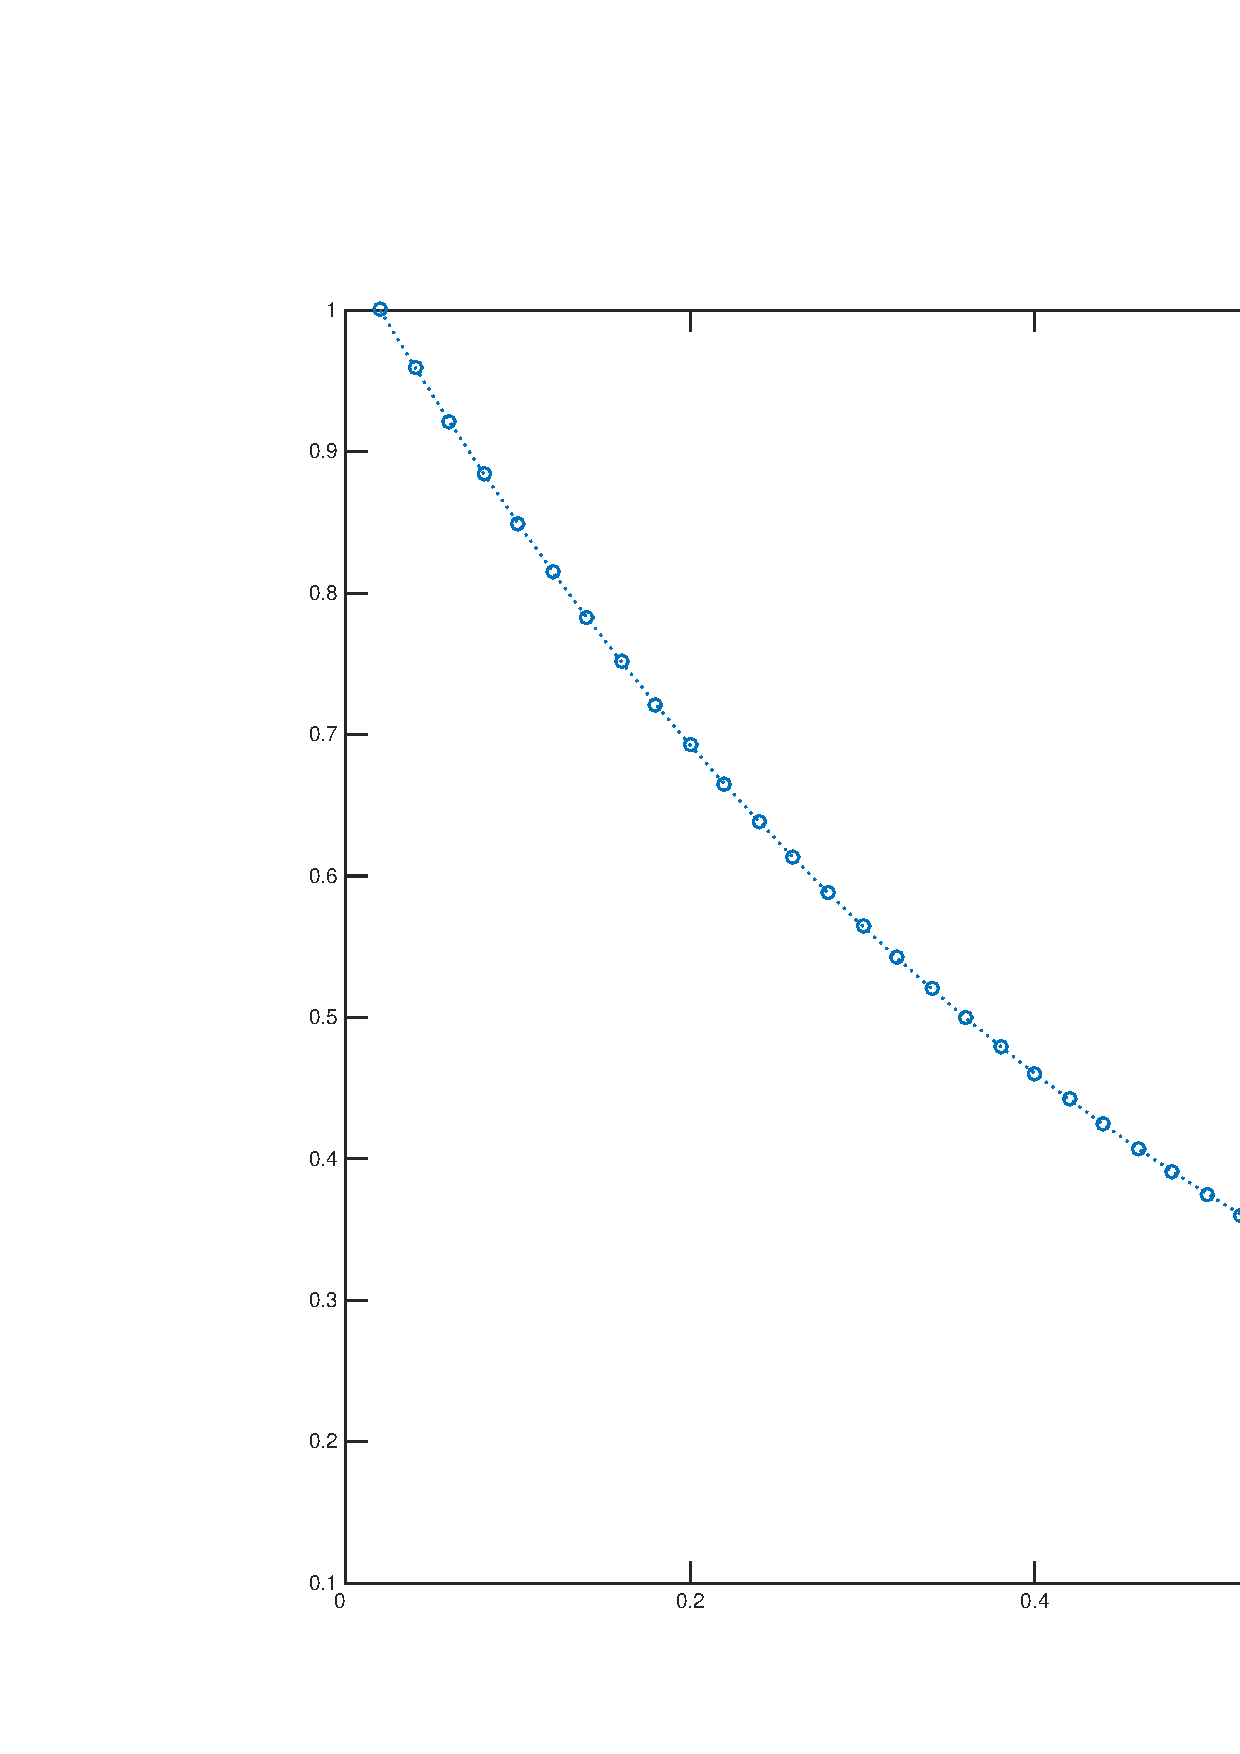
\includegraphics[width=5.5in]{1.jpg}}

\centerline{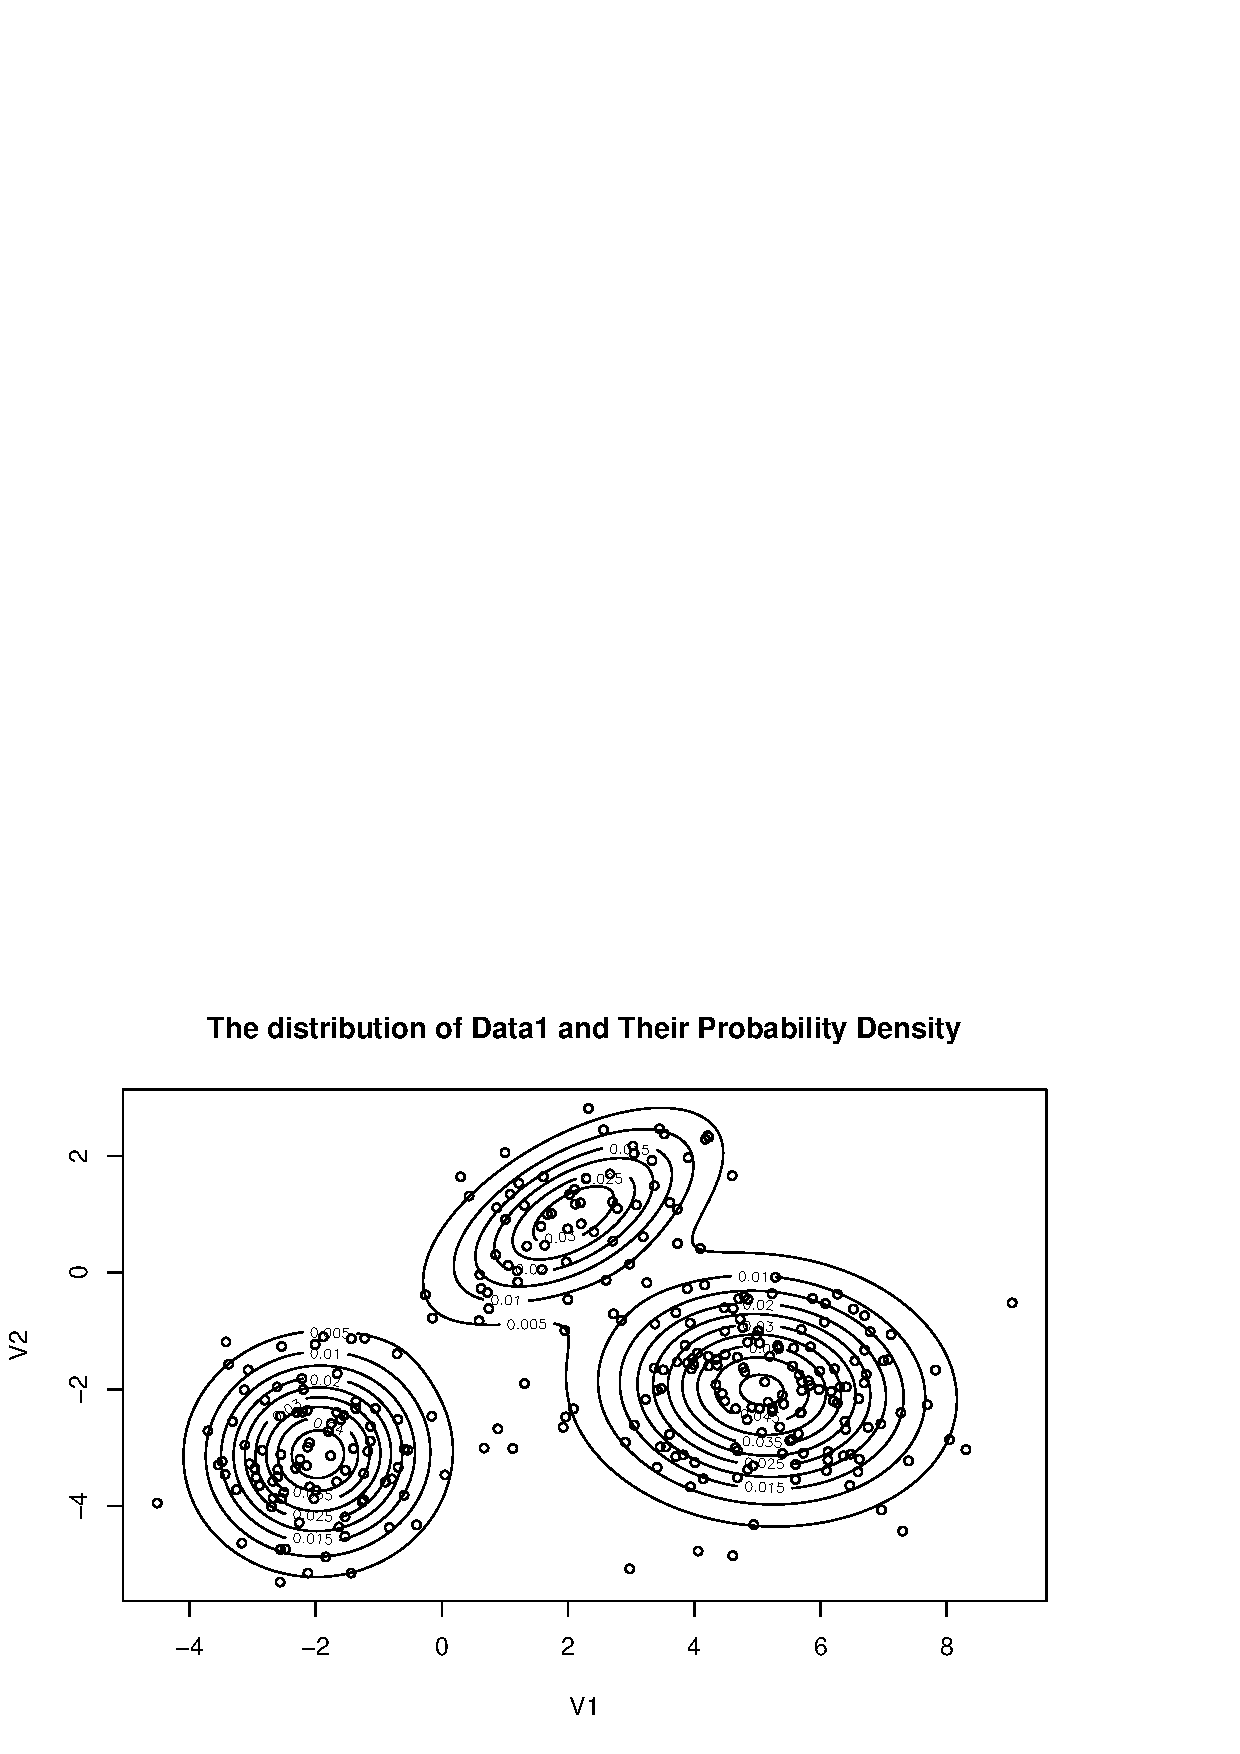
\includegraphics[width=4in]{2.jpg}}

\centerline{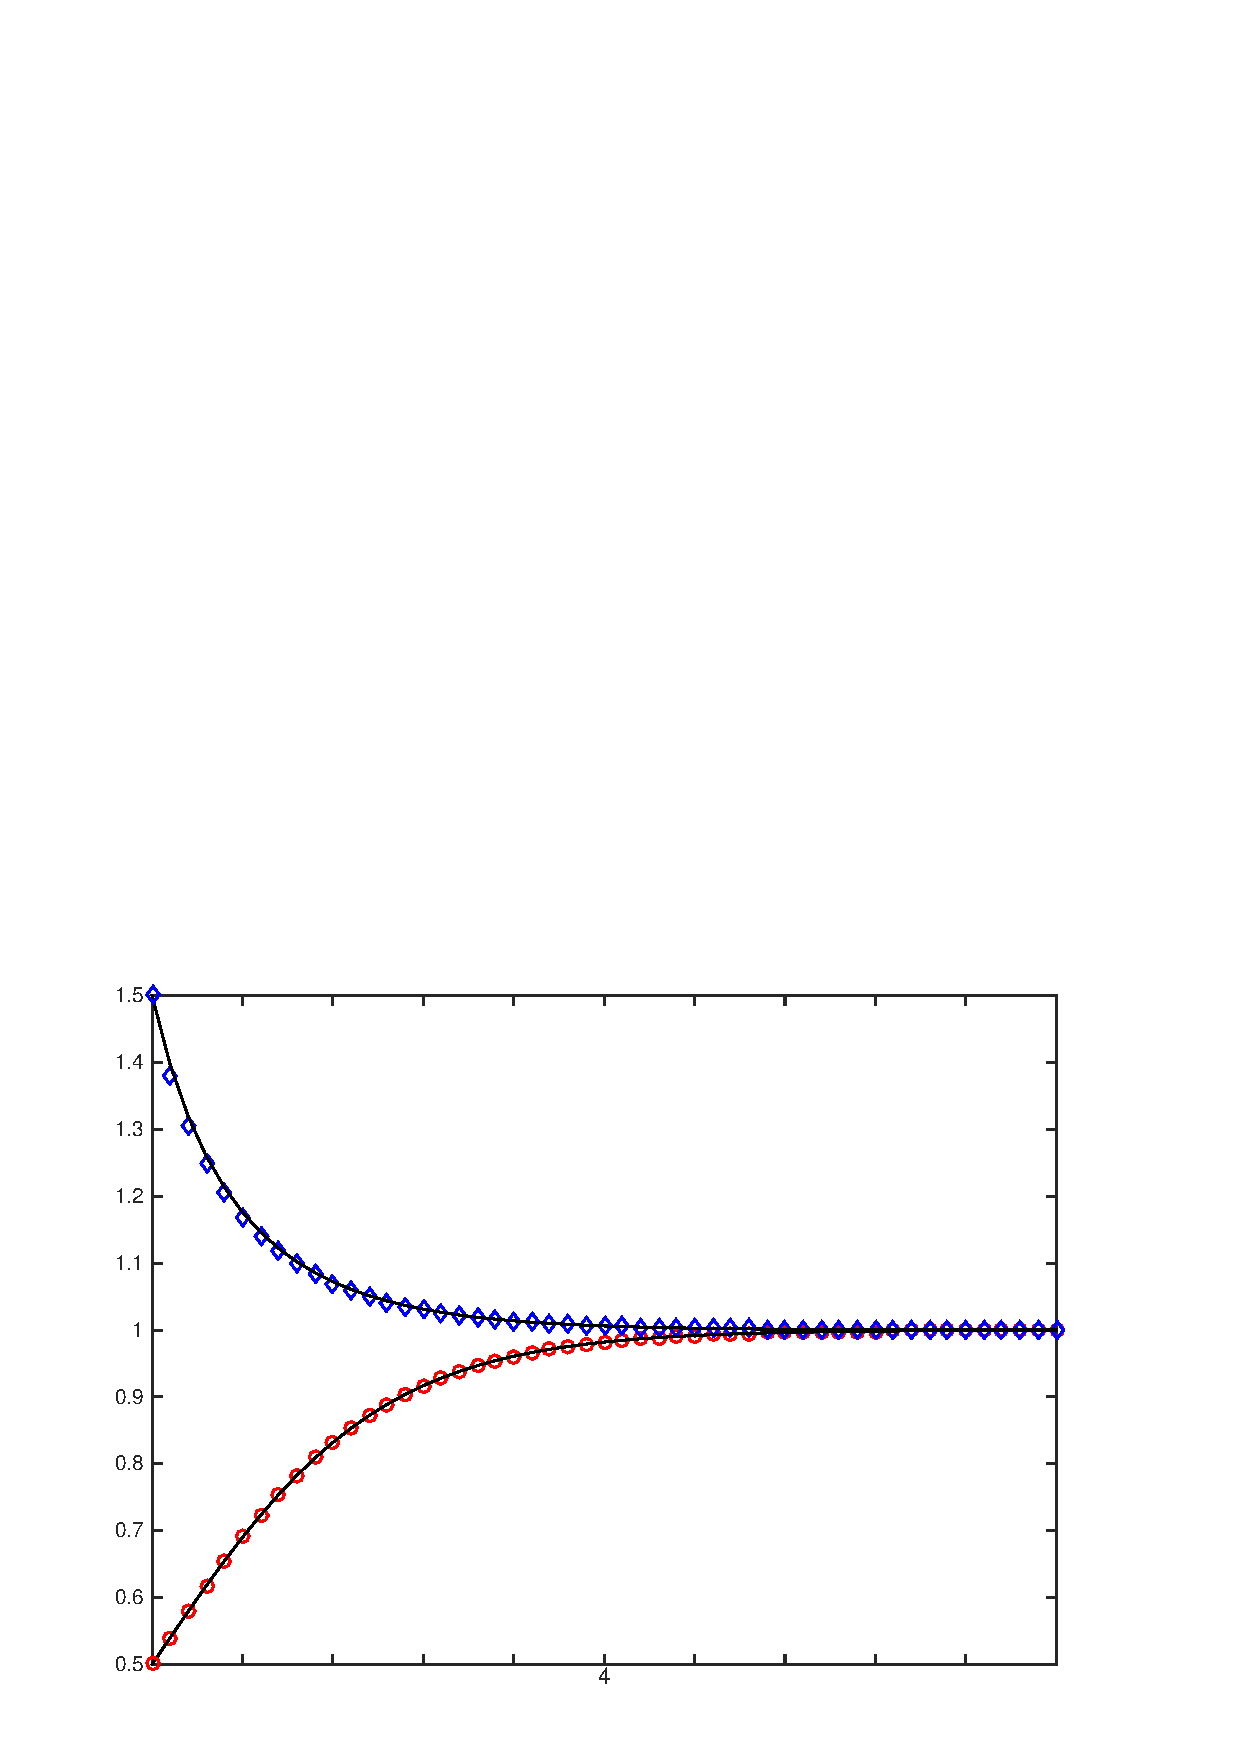
\includegraphics[width=4in]{3.jpg}}

对于Chebyshev插值点与等距插值点的选取,其Lebesgue常数分别为
\[
\Lambda^{\mbox{Ch}}_N=O (\ln N),\Lambda^{\mbox{eq}}_N=O (\frac{2^N}{N \ln N})
\]

对于等距节点插值,其Lebesgue常数\(\Lambda^{\mbox{eq}}_N\)可,能会出现指数增长,这样就造成对于函数\(f(x)= \displaystyle \frac{1}{1+25x^2}\)的等距节点插值只对\(x=0\)处逼近的较好,并且出现Runge现象,等距节点插值的误差在中间部分最小,靠近端点处越来越大。而Chebyshev插值点的Lebesgue常数增长要慢得多,而随着拟合多项式的次数增加,Chebyshev多项式拟合表现出更好的逼近性。



\item 用各种求积公式计算\(x^2\)的积分,看可以精确计算几次多项式

编写程序如下:

\begin{lstlisting}[language=Matlab,keywordstyle=\color{blue!70},commentstyle=\color{red!50!green!50!blue!50},frame=shadowbox, rulesepcolor=\color{red!20!green!20!blue!20}] ]
I=zeros(7,6);
for n=1:7
    f=@(x) x^n;
    
    %精确值
    I(n,1)=int(x^n,0,1);
    
    %中点公式
    I(n,2)=f(1/2);
    
    %梯形公式
    I(n,3)=1/2*(f(0)+f(1));
    
    %Simpson公式
    I(n,4)=1/6*(f(0)+4*f(1/2)+f(1));
    
    %3/8规则
    for i=0:3
        xx(i+1)=i/3;
    end
    I(n,5)=1/8*(f(xx(1))+3*f(xx(2))+3*f(xx(3))+f(xx(4)));
    
    %Cotes公式
    for i=0:4
        yy(i+1)=i/4;
    end
    I(n,6)=1/90*(7*f(yy(1))+32*f(yy(2))+12*f(yy(3))+32*f(yy(4))+7*f(yy(5))); 
end
\end{lstlisting}

得到I即下表

\begin{tabular}{|c|c|c|c|c|c|c|}
\hline
\multicolumn{7}{|c|}{用Newton公式计算\(x^n\)的积分}\\ 
\hline
&精确值 &中点公式 &梯形公式 &Simpson公式 &\(\frac{3}{8}\)规则 &Cotes公式 \\
\hline
\(x^1\) &0.5000 &\bf 0.5000 &\bf 0.5000 &0.5000 &0.5000 &0.5000 \\
\hline
\(x^2\) &0.3333 &0.2500 &0.5000 & \bf 0.3333 &0.3333 &0.3333 \\
\hline
\(x^3\) &0.2500 &0.1250 &0.5000 & \bf 0.2500 &\bf 0.2500 &0.2500 \\
\hline
\(x^4\) &0.2000 &0.0625 &0.5000 &0.2083 &0.2037 &\bf 0.2000 \\
\hline
\(x^5\) &0.1667 &0.0313 &0.5000 &0.1875 &0.1759 &\bf 0.1667 \\
\hline
\(x^6\) &0.1429 &0.0156 &0.5000 &0.1771 &0.1584 &0.1432 \\
\hline
\(x^7\) &0.1250 &0.0078 &0.5000 &0.1719 &0.1471 &0.1263 \\
\hline
\end{tabular}


从表中可以看出中点公式、梯形公式、Simpson公式、\(\frac{3}{8}\)规则,Cotes公式可以分别精确计算到第1,1,3,3,5次多项式。

再用Gauss求积公式计算\(x^n\)的积分

\begin{lstlisting}[language=Matlab,keywordstyle=\color{blue!70},commentstyle=\color{red!50!green!50!blue!50},frame=shadowbox, rulesepcolor=\color{red!20!green!20!blue!20}] ]
%高斯求积公式计算x^n积分
I=zeros(7,6);
for n=1:7
    syms x
    f=@(x) x.^n;
    %精确值
    I(n,1)=int(x^n,0,1);
    %1点
    for j=0:4
        [x,w]=legendregauss(j);
        I(n,j+2)=1/2*sum(w*f(1/2*x+1/2));
    end
end
\end{lstlisting}

得到下表:

\begin{tabular}{|c|c|c|c|c|c|c|}
\hline
\multicolumn{7}{|c|}{用Newton公式计算\(x^n\)的积分}\\ 
\hline
&精确值 &1点 &2点 &3点 &4点 &5点 \\
\hline
\(x^1\) &0.5000 &\bf 0.5000 &\ 0.5000 &0.5000 &0.5000 &0.5000 \\
\hline
\(x^2\) &0.3333 &0.2500 &\bf 0.3333&  0.3333 &0.3333 &0.3333 \\
\hline
\(x^3\) &0.2500 &0.1250 &\bf 0.2500 & \ 0.2500 &\ 0.2500 &0.2500 \\
\hline
\(x^4\) &0.2000 &0.0625 &0.1944 &\bf 0.2000 &0.2000 & 0.2000 \\
\hline
\(x^5\) &0.1667 &0.0313 &0.1528&\bf 0.1667 &0.1667 & 0.1667 \\
\hline
\(x^6\) &0.1429 &0.0156 &0.1204 &0.1425 &\bf 0.1429&0.1429 \\
\hline
\(x^7\) &0.1250 &0.0078 &0.0949 &0.1238 &\bf 0.1250 & 0.1250 \\
\hline
\end{tabular}
  





















\end{enumerate}
\end{document}